\documentclass{article}
\usepackage{graphicx} % Required for inserting images
\usepackage{amsfonts}


\title{25.01.14 ATMS with Product of All Keys}
\author{Xun Zhang \quad \quad Wuyun Siqin \quad \quad Bingsheng Zhang \\ 
Zhejiang University, CHN \\
22221024@zju.edu.cn \quad 3210101763@zju.edu.cn \quad bingsheng@zju.edu.cn}
\date{January 14 2025}

\begin{document}

\maketitle

\section{ATMS with Product}

First we introduce the original version of a multisignature-based t-ATMS construction:

Given $d$ individual signatures $\sigma_1, \ldots, \sigma_d$, created using secret keys belonging to (not
necessarily unique) public keys $vk_1, \ldots, vk_d$ can be combined into a multisignature $\sigma = \prod_{i=1}^d \sigma_i$ that can then be verified using an aggregated public key $avk = \prod_{i=1}^d vk_i$.

Assuming $S$ is a set and $\langle S \rangle$ is a a Merkle-tree commitment to the set. There are some functions:

\begin{itemize}
    \item $\mathsf{AKey}$: given a sequence of public keys $\mathcal{VK} = \{vk_i\}_{i=1}^n$, returns $avk = (\prod_{i=1}^d vk_i, \langle \mathcal{VK}\rangle)$.
    \item $\mathsf{ACheck}(\mathcal{VK},avk)$: simply recomputes it to verify $avk$.
    \item $\mathsf{ASig}$: takes the message $m$, $d$ pairs of signatures with their respective public keys $\{\sigma_i, vk_i\}_{i=1}^d$ and $n-d$ additional public keys $\{\widehat{vk_i}\}_{i=1}^{n-d}$ and produces an aggregate signature:
    \[
    \sigma = \left ( \prod_{i=1}^d \sigma_i , \{\widehat{vk_i}\}_{i=1}^{n-d}, \{\pi_{\widehat{vk_i}}\}_{i=1}^{n-d}\right )
    \]
    where $\{\pi_{\widehat{vk_i}}\}_{i=1}^{n-d}$ denotes the (unique) inclusion proof of $\{{\widehat{vk_i}}\}_{i=1}^{n-d}$ in the Merkle commitment.
    \item $\mathsf{AVer}$: takes a message $m$, an aggregate key $avk$, and an aggregate signature $\sigma$ parsed as above and does the following: 
    \begin{enumerate}
        \item verifies that each of the public keys $\widehat{vk_i}$ indeed belongs to a different leaf
        in the commitment $\langle \mathcal{VK}\rangle$ in $avk$ using membership proofs $\pi_{\widehat{vk_i}}$.
        \item computes $avk'$ by dividing the first part of $avk$ by $\prod_{i=1}^{n-d} \widehat{vk_i}$.
        \item returns true if and only if $d \geq t$ and the first part of $\sigma$ verifies as a $\Pi_\mathsf{MGS}$-signature
        under $avk'$
    \end{enumerate}
\end{itemize}


\section{Relations}

In a SNARK version of ATMS with product(original ATMS), we have a $avk$ as the root of a Merkle tree containing $\mathcal{VK}$. And let $S' = \{s_i\}$ be the signatures generated by a sequence $\mathcal{VK}'$ containing keys in $\mathcal{VK}$. The signing algorithm reconstructs the Merkle tree from
$\mathcal{VK}$ and determines the membership proof $\pi_i$ for each $vk_i \in \mathcal{VK}'$. 

The the statements of SNARK is $x = (avk,m)$, and the witness of SNARK is $w = \{\pi_i, (s_i,vk_i)\}_{i \in S'}$. The SNARK prove the following relations:
\begin{itemize}
    \item For all $i$, the signature verifying algorithm $\mathsf{Ver}(vk_i,m,s_i)$ returns true.
    \item For all $i$, proof $\pi_i$ is a valid Merkle path proof pointing to a unique leaf.
    \item $|S'| \geq t$.
\end{itemize}

This is very similar to the code implemented by Inigo, but the original code replace the Merkle tree by a straight hash.


\section{SNARK-based ATMS Implementation}

According to the relations mentioned in the paper, the code implementation is as following:

\vspace{0.5cm}

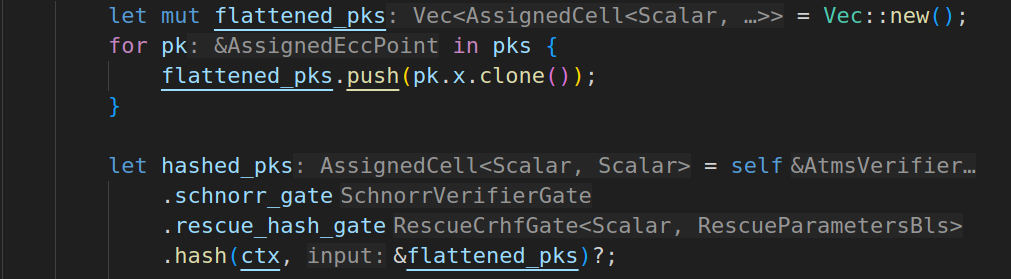
\includegraphics[width=1\linewidth]{inigo_atms_code_keyhash.png}
\vspace{0.1cm}

Compute a straight hash of all public keys firstly, and compare it to the public commitment.

Then, just as described in the paper, we verify the individual signature one by one. And if there exits a signature corresponding to a public keys, which can also be verified, we add the counter(to compute the threshold).


\vspace{0.5cm}

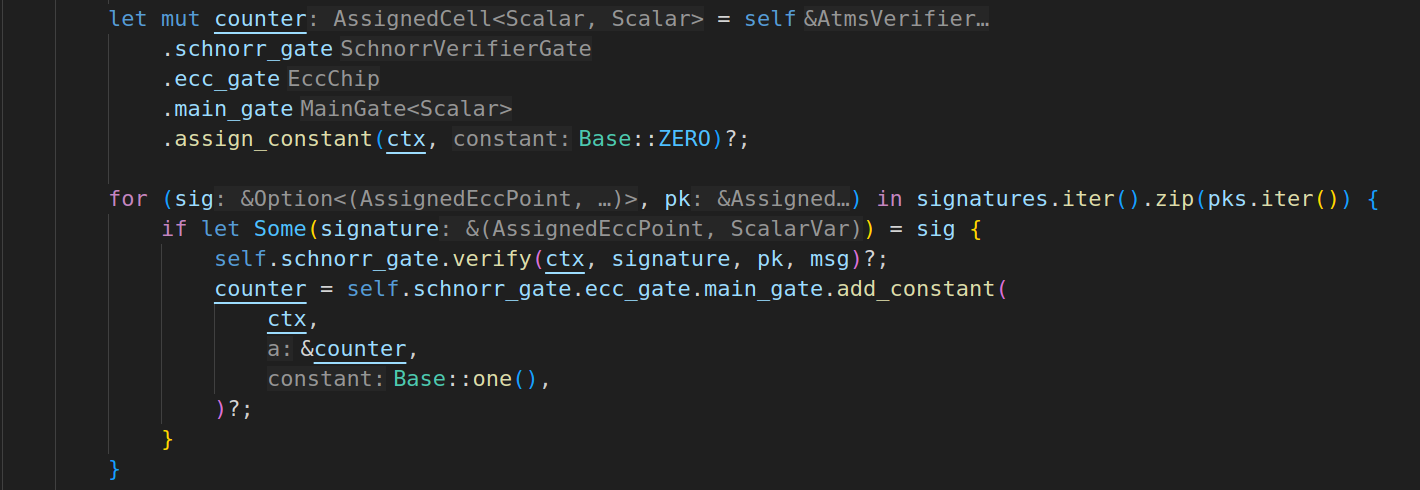
\includegraphics[width=1\linewidth]{inigo_atms_code_verify.png}
\vspace{0.1cm}


Finally we constraint the counter to be equal with threshold.

\vspace{0.5cm}

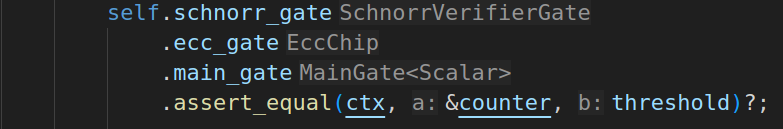
\includegraphics[width=1\linewidth]{inigo_atms_code_threshold.png}
\vspace{0.1cm}


\section{New Approach}


If we use the settings in the ATMS paper, which means that there do exit a Merkle tree that commits $\mathcal{VK}$. And we need a product of all public keys $ ivk = \prod_{i=1}^n vk_i$ at first. Now, let the $avk$ be aggregated public key $avk =  \prod_{i=1}^d vk_i$, and $\sigma = \prod_{i=1}^n \sigma_i$ be the aggregated signature.

Then the The the statements of SNARK is $x = (avk,ivk,m,\sigma)$, and the witness of SNARK is $w = \{\{\pi_i, vk_i\}_{i \notin S'}, \{\sigma_i\}_{i \in S'}\}$. The SNARK prove the following relations:

\begin{itemize}
    \item $avk = ivk - \prod_{i=1}^{n-d} vk_i$.
    \item For all $i$, proof $\pi_i$ is a valid Merkle path proof pointing to a unique leaf.
    \item $\sigma = \prod_{i=1}^d \sigma_i$.
    \item The signature verifying algorithm $\mathsf{Ver}(avk,m,
    \sigma)$ returns true.
\end{itemize}


This is a normal multisignature-like proving approach.


\section{Advantage}

The SNARK-based ATMS implementation use Schnorr signature as its core signature scheme, but when we turn to \textbf{BLS} signature, the proving cost will increase rapidly.

Assuming the threshold is $d$, the original approach in paper need to prove(in BLS setting):

\begin{itemize}
    \item $d$ BLS signature verification.
\end{itemize}

Which means it need to prove $d$ times of pairing check, it is very costly.


In our approach, we need to prove:

\begin{itemize}
    \item Product of unused keys, signatures and the result of $avk$.
    \item $n-d$ times of Merkle path verification.
    \item $1$ BLS signature verification.
\end{itemize}


The main cost is Merkle path verification, it may can be optimized by our shuffle argument.

\section{Test Result}

Below are our test results. We continued using the same parameter settings as before, meaning we signed with half of the total number of keys. 

\begin{table}[htbp]
    \centering
    \renewcommand{\arraystretch}{1.1} % 增加行间距
    \setlength{\tabcolsep}{10pt}      % 增加列间距
    \begin{tabular}{c|c|c|c} \hline
        \textbf{num} & \textbf{proof\_time} & \textbf{proof\_size} & \textbf{verify\_time} \\ \hline
        16 of 32    & 29.24s  & 13152  & 15.07ms  \\
        32 of 64    & 30.75s  & 14528  & 12.93ms  \\
        64 of 128   & 36.50s  & 17984  & 16.33ms  \\
        128 of 256  & 51.53s  & 25600  & 16.60ms  \\
        256 of 512  & 82.75s  & 41856  & 23.04ms  \\
        512 of 1024 & 147.84s & 76672  & 35.33ms  \\
        1024 of 2048 & 289.60s & 151488 & 56.85ms  \\ \hline
    \end{tabular}
    \label{tab:example_benchmark_selected}
\end{table}

Currently, the main bottleneck lies in the hash verification process used for Merkle tree validation. However, we need to adjust our parameters. Under the actual ATMS configuration, about two-thirds of the keys would be used for signing. Because the Merkle paths to be verified correspond to keys that are not signed, the real-world verification time will be lower than the current test results. So we need further testing.

\newpage

The figure below shows that, under the current parameter settings, both the proving time and the verification time increase linearly with the number of keys.
\begin{figure}[htbp]
    \centering
    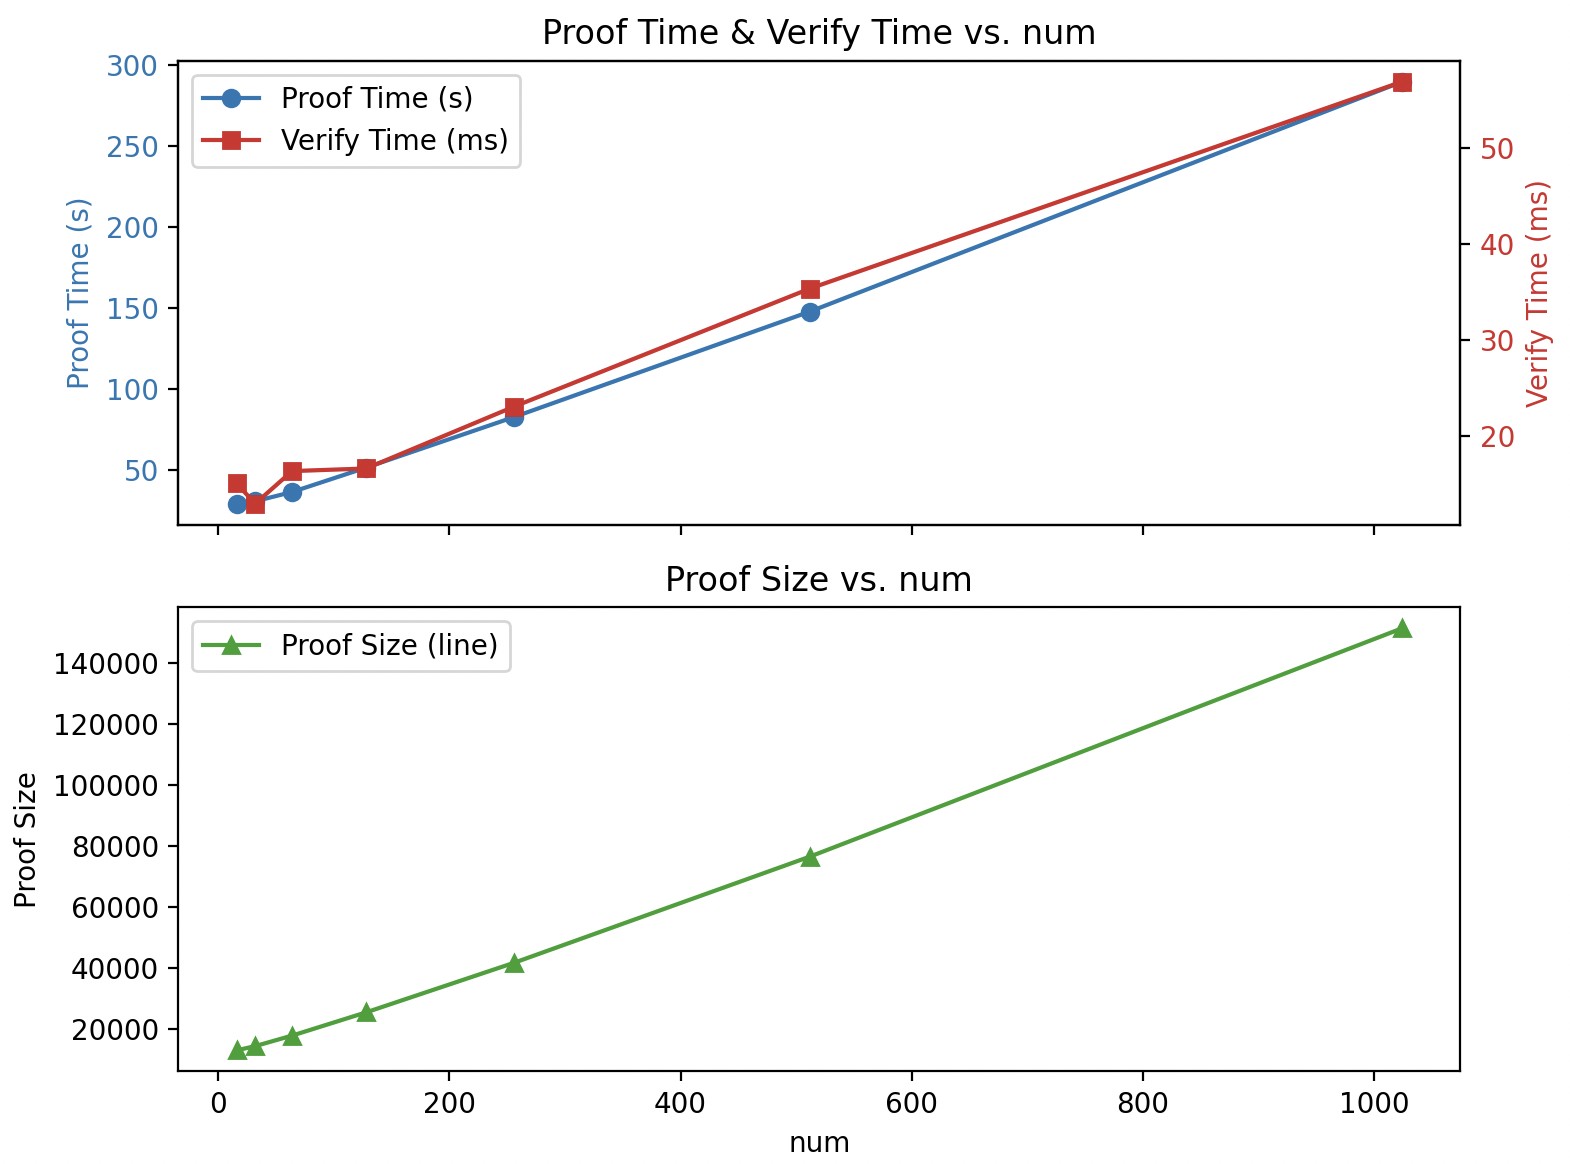
\includegraphics[width=1\linewidth]{test2.png}
    % \caption{Enter Caption}
    \label{fig:enter-label}
\end{figure}

\end{document}
